\section{Omitted Proofs}\label{app:proofs}

This appendix collects the proofs deferred from the main text. Statements are
those of the corresponding numbered results above.

\subsection{Proof of Theorem~\ref{thm:decomp}}\label{app:decomp}

\begin{proof}
Write $V_t := V(S_t)$. The It\^o--L\'evy formula for jump-diffusion processes \cite[Prop.~8.14]{cont2003financial} applied to $V$, with $S$ satisfying \eqref{eq:merton}, gives
\begin{align*}
V(S_t) - V(S_0) =\;& \int_0^t V'(S_{s-})\,dS_s \\
&+ \tfrac{1}{2}\int_0^t V''(S_{s-})\,\sigma^2 S_{s-}^2 \,ds \\
&+ \sum_{0 < s \leq t} \!\Big[V(S_s) - V(S_{s-}) - V'(S_{s-})(S_s - S_{s-})\Big].
\end{align*}
Substituting into \eqref{eq:lvrdef},
\begin{equation}\label{eq:lvr-itl}
\mathrm{LVR}(t) \;=\; -\tfrac{1}{2}\int_0^t V''(S_{s-})\,\sigma^2 S_{s-}^2 \, ds \;-\; \sum_{0 < s \leq t}\!\Big[V(S_s) - V(S_{s-}) - V'(S_{s-})\,\Delta S_s\Big].
\end{equation}
Both terms are nonnegative because $V$ is concave: $V''<0$ and $V(S_s) \leq V(S_{s-}) + V'(S_{s-})\Delta S_s$.

\emph{Diffusion term.} With $V''(P) = -x(P)/(2P)$ and $V(P) = 2\sqrt{LP}$, $-\tfrac{1}{2} V''(P) \sigma^2 P^2 = \tfrac{\sigma^2}{4} P\,x(P) = \tfrac{\sigma^2}{4} \sqrt{L P} = \tfrac{\sigma^2}{8} V(P)$.

\emph{Jump term.} At a jump time $\tau$ with $S_\tau = S_{\tau-} e^{J}$, writing $r := e^J$,
\begin{align*}
V(S_\tau) - V(S_{\tau-}) - V'(S_{\tau-})\,\Delta S_\tau
&= 2\sqrt{L S_{\tau-}}\Big[\sqrt{r} - 1 - \tfrac{r-1}{2}\Big] \\
&= -\sqrt{L S_{\tau-}}\,(\sqrt{r}-1)^2 \;=\; -\tfrac{1}{2}\,V(S_{\tau-})\,(e^{J/2} - 1)^2.
\end{align*}
The jump contribution to \eqref{eq:lvr-itl} is therefore $\sum_{\tau} \tfrac{1}{2}\,V(S_{\tau-})\,(e^{J_\tau/2} - 1)^2$. By the marked-Poisson compensator formula \cite[Prop.~8.8]{cont2003financial}, and using the independence of jump marks $J$ from the predictable filtration $\mathcal{F}_{\tau-}$,
\[
\E\!\Big[\sum_{\tau \leq t} \tfrac{1}{2}V(S_{\tau-})(e^{J_\tau/2}-1)^2\Big] \;=\; \tfrac{\lambda}{2}\,\E[(e^{J/2}-1)^2]\cdot\E\!\Big[\int_0^t V(S_{s-})\,ds\Big],
\]
so the expected rate at state $V_t$ is $\tfrac{\lambda}{2} V_t \E[(e^{J/2}-1)^2]$.

\emph{Moments.} Expanding $(e^{J/2}-1)^2 = e^{J} - 2 e^{J/2} + 1$ and taking expectations under $J \sim \mathcal{N}(m,\delta^2)$ gives the bracket in Theorem~\ref{thm:decomp}, nonnegative as the expectation of a square and vanishing only in the degenerate case $J\equiv 0$.
\end{proof}

\subsection{Proof of Lemma~\ref{lem:F}}\label{app:F}

\begin{proof}
By \eqref{eq:rate-stationary} with the quadratic loss and \eqref{eq:pi0},
$\ell_{\mathrm{diff}} = \tfrac{V}{8\dt}\E_\pi[(|z|-\gamma)_+^2] = \tfrac{V}{8\dt}\cdot2\int_0^\infty u^2 c\,e^{-\theta u}du = \tfrac{V}{8\dt}\cdot 4c/\theta^3 = \tfrac{V}{8\dt}\cdot 2/(\theta^2(1+\eta))$,
and $\theta^2 = 2/(\sigma^2\dt)$ gives $2/(\theta^2\dt) = \sigma^2$, so $\ell_{\mathrm{diff}} = \tfrac{\sigma^2V}{8}(1+\eta)^{-1}$ with $\eta=\sqrt2 \kappa$.
\end{proof}

\subsection{Proof of Lemma~\ref{lem:G}}\label{app:G}

\begin{proof}
Jumps and blocks are independent Poisson processes, so the jump count over an inter-block interval is geometric: with $\rho:=\lambda\dt/(1+\lambda\dt)$, exactly one jump has probability $(1-\rho)\rho$ and two or more probability $\rho^2$, both exactly. The multi-jump contribution is carried in Proposition~\ref{prop:error}. Conditional on one jump of mark $J$ with $|J|>\gamma$, the arbitrageur executes at the next block, leaving the pool's marginal log-price at distance $\gamma$ from the external price and capturing the residual concavity gap; for the quadratic surrogate of \eqref{eq:rate-stationary} (with $\xi := |J|-\gamma$) this loss is $\tfrac{V}{8}(|J|-\gamma)^2$. The pre-block mispricing is in fact $z = M + X + J$, with $M\in[-\gamma,\gamma]$ the state carried in and $X$ the interval's diffusive increment; write $Y := M+X$ for the pair. Dropping $Y$ is the first of two approximations here. The second is the rate: one-jump intervals occur at the thinned block rate $(1-\rho)\rho/\dt = \lambda(1+\lambda\dt)^{-2}$, so the exact one-jump contribution is $\lambda(1+\lambda\dt)^{-2}\,V\,G(\gamma;m,\delta^2)$ before the interaction correction; charging instead at the full jump rate $\lambda$ --- which is what keeps the term free of $\dt$ --- gives the separated contribution $\lambda V \cdot G(\gamma;m,\delta^2)$. Both deficits, interaction and thinning, are bounded in Proposition~\ref{prop:error}. Strict monotonicity in $\gamma$ follows since $(|j|-\gamma)^2 \1\{|j|>\gamma\}$ is strictly decreasing in $\gamma$ pointwise on the support.
\end{proof}

\subsection{Proof of Proposition~\ref{prop:error}}\label{app:error}

\begin{proof}
Write $u:=\lambda\dt$ and $\rho:=u/(1+u)$, so the jump count over an inter-block interval is geometric, $\Prob(N{=}k)=\rho^k(1-\rho)$. On intervals with $k\ge2$ jumps, $g(z)\le z^2$ gives a loss at most $\tfrac{V}{8}\big(\E[M^2]+\E[X^2\mid N{=}k]+k\delta^2\big)$, with $\E[M^2]\le\gamma^2$ pathwise and, since $T\mid N{=}k\sim\mathrm{Gamma}(k{+}1,\dt^{-1}{+}\lambda)$, $\E[X^2\mid N{=}k]=\sigma^2(k{+}1)\dt/(1+u)$. The geometric sums over $k\ge2$ are $\sum\rho^k(1-\rho)=\rho^2$, $\sum k\rho^k(1-\rho)=\rho^2(2-\rho)/(1-\rho)$ and $\sum(k{+}1)\rho^k(1-\rho)=\rho^2(3-2\rho)/(1-\rho)$; dividing by $\dt$ and relaxing via $\rho^2/\dt\le\lambda^2\dt$, $\rho^2(2-\rho)/\big((1-\rho)\dt\big)\le2\lambda^2\dt$ and $\rho^2(3-2\rho)/\big((1-\rho)(1+u)\dt\big)\le3\lambda^2\dt$ bounds their contribution by $\tfrac{V\lambda^2\dt}{8}(\gamma^2+3\sigma^2\dt+2\delta^2)$, the last term of the display. Conditional on exactly one jump, write the pre-block mispricing as $Y+J$, with $Y$ independent of the mark $J$. Convexity of $g$ with $2$-Lipschitz gradient gives $0\le g(y+j)-g(j)-g'(j)y\le y^2$, so taking expectations,
\[
0 \;\le\; \E[g(Y+J)]-\E[g(J)] - \E[g'(J)]\,\E[Y] \;\le\; \E[Y^2\mid N{=}1].
\]
Symmetry gives $\E[Y]=0$, so the cross term drops. The single-jump contribution to the rate is $\tfrac{V}{8}\,\lambda(1+u)^{-2}\,\E[g(Y+J)]$, since $\Prob(N{=}1)/\dt=\lambda(1+u)^{-2}$, against the separated charge $\tfrac{V}{8}\,\lambda\,\E[g(J)]$; their difference splits as
\[
\tfrac{V}{8}\,\lambda(1+u)^{-2}\big(\E[g(Y{+}J)]-\E[g(J)]\big) \;-\; \tfrac{V}{8}\,\lambda\big[1-(1+u)^{-2}\big]\,\E[g(J)].
\]
The first piece is the interaction: it is \emph{nonnegative} by the display above, and since $(1+u)^{-2}\le1$ it is at most $\tfrac{\lambda V}{8}\E[Y^2\mid N{=}1]$. The second is the thinning deficit: it is nonpositive, and $1-(1+u)^{-2}\le2u$ bounds it below by $-2\lambda^2\dt\,VG_\nu(\gamma)$, the third term on the lower side --- the jumps that thinning removes from single-jump intervals land in multi-jump intervals, whose losses are carried, nonnegative, on the upper side. For the interaction's moments, conditioning on a jump size-biases the interval, $T\mid N{=}1\sim\mathrm{Gamma}(2,\dt^{-1}+\lambda)$, whence $\E[X^2\mid N{=}1]\le2\sigma^2\dt$, while $\E[M^2]\le\gamma^2$ because the post-block state lies in the band by construction --- no property of its stationary law is used. Conditioning on $N{=}0$ gives weight $(1+u)^{-1}$ and makes the inter-block increment Laplace with rate $\theta\sqrt{1+u}$, so by the computation of Lemma~\ref{lem:F} that contribution is exactly $\ell_{\mathrm{diff}}\,R$ with $R = (1+\eta)\big/\big[(1+u)^2\big(1+\eta\sqrt{1+u}\big)\big]$. Here $R\le1$, since $(1+u)^2\ge1$ and $1+\eta\sqrt{1+u}\ge1+\eta$; and $R\ge1-\tfrac52u$, since $(1+u)^{-2}\ge1-2u$ and $\sqrt{1+u}\le1+u/2$ give $(1+\eta)/(1+\eta\sqrt{1+u})\ge1-\tfrac{\eta u}{2(1+\eta)}\ge1-u/2$, and $(1-2u)(1-u/2)=1-\tfrac52u+u^2\ge1-\tfrac52u$. The block-clock deficit therefore lies between $0$ and $\tfrac52\lambda\dt\,\ell_{\mathrm{diff}}$, with no expansion. For the stationary-law term, couple the two chains on the same block times and Brownian path: they agree unless a jump lands, and $\Prob(N\ge1)=1-\E[e^{-\lambda T}]=\lambda\dt/(1+\lambda\dt)$ for $T\sim\mathrm{Exp}(1/\dt)$, so $\sup_m\|K(m,\cdot)-K_0(m,\cdot)\|_{\mathrm{TV}}\le\lambda\dt/(1+\lambda\dt)\le\lambda\dt$ and, telescoping, $\|K^n-K_0^n\|\le n\lambda\dt$. If $n_*$ is a mixing time for $K_0$, in the sense $\sup_{m,m'}\|K_0^{n_*}(m,\cdot)-K_0^{n_*}(m',\cdot)\|\le\tfrac12$, then $\|\pi-\pi_0\|\le2n_*\lambda\dt$. Condition \eqref{eq:mix} is the form the band's relaxation takes: an interval of width $2\gamma$ carrying a walk of step variance $2/\theta^2$ has diffusive relaxation time $4\eta^2/\pi^2$, and the additive $1$ keeps it meaningful for the integer $n_*$ at small $\eta$. Establishing \eqref{eq:mix} for the clipped Laplace kernel itself --- sticky rather than reflecting boundaries, discrete rather than diffusive at finite $\eta$ --- is not attempted here. Since $K_0$ depends on $(\gamma,\sigma,\dt)$ only through $\eta$, and not at all on $\lambda$, \eqref{eq:mix} is a condition on $\eta$ alone, and it is checked numerically over the whole empirically relevant range: every block time from $50$~ms to $12$~s, every volatility in $[0.30,1.50]$, every jump intensity, and every Uniswap fee tier from $1$ to $100$~bps --- jointly, $\eta$ from $0.15$ to $1.2\times10^{3}$. Over that range the ratio $n_*/(1+\eta^2)$ peaks at $1.27$ near $\eta=0.8$, against the $2$ that \eqref{eq:mix} asks for, and settles near $0.38$ in the fast-block, wide-band corner, so the margin is smallest where the band is narrow relative to a block's diffusion and only widens from there. Since $\eta^2=2\gamma^2/(\sigma^2\dt)$, \eqref{eq:mix} gives $\|\pi-\pi_0\|\le 2C\lambda\dt+4C\lambda\gamma^2/\sigma^2$. Finally the per-block diffusion loss $\phi(m)=\tfrac{V}{8}\E[(|m+X|-\gamma)_+^2] = \tfrac{V}{8\theta^2}\,2e^{-\eta}\cosh(\theta m)$ has $\mathrm{osc}(\phi)=\tfrac{V}{8\theta^2}(1-e^{-\eta})^2\le V\sigma^2\dt/16$, and $\mathrm{osc}(\phi)\,\|\pi-\pi_0\|/\dt \le \tfrac{\lambda V}{4}(2\gamma^2+\sigma^2\dt)$ at $C=2$. Finally $\mathcal{E}_{\mathrm{curv}} = \tfrac{V}{2}\E_\pi[\rho(\xi)]$ is nonnegative by \eqref{eq:rhosign}, $\pi$ being symmetric.
\end{proof}

\subsection{Proof of Theorem~\ref{thm:floor}}\label{app:floor}

\begin{proof}
Over an inter-block interval carrying $N$ jumps with marks $J_1,\dots,J_N$, the pre-block mispricing is $z = Y + \sum_{k\le N}J_k$. Three steps, each an inequality in the same direction.

\emph{(i) Concavity residual.} At $m=0$ the law of $z$ is symmetric, so $\E_\pi[h(\xi)] \ge \tfrac{V}{8}\E_\pi[\xi^2] = \tfrac{V}{8}\E_\pi[g(z)]$ by \eqref{eq:rhosign}. It therefore suffices to bound the convex surrogate from below.

\emph{(ii) Interaction.} All the next step needs is $\E[Y\mid N{=}k,\,\sum J = s]=0$. $M$ is fixed by the previous block and so is independent of this interval's jumps, with $\E[M]=0$ by symmetry; the Brownian path is independent of the Poisson process and its marks, and $X\mid T\sim\mathcal N(0,\sigma^2T)$ is mean-zero conditionally on $T$, a property preserved by averaging over any law of $T$, in particular the size-biased one induced by conditioning on $N$. Conditional Jensen applied to the convex $g$ then gives $\E[g(Y+s)\mid N{=}k,\,\sum J = s] \ge g(s)$, hence $\E[g(z)\mid N{=}k] \ge \E[g(\sum_{k}J)]$. Dropping the interaction can only lower the loss.

\emph{(iii) Aggregation.} This is the hypothesis, and Merton satisfies it: $\sum_{1}^{k}J \sim \mathcal N(0,k\delta^2)$, so by \eqref{eq:Gclosed} and the monotonicity of $\Psi$,
\[
\E\big[g(\textstyle\sum_1^k J)\big] \;=\; k\delta^2\,\Psi\!\big(\tfrac{\gamma}{\delta\sqrt k}\big) \;\ge\; k\delta^2\,\Psi\!\big(\tfrac{\gamma}{\delta}\big) \;=\; k\,\E[g(J)],
\]
since $\gamma/(\delta\sqrt k)\le\gamma/\delta$. Several jumps in one interval are cleared by a single trade, and that trade costs at least as much as clearing them one at a time.

Combining, and using $\E[N]=\lambda\dt$ exactly for a Poisson jump process observed over an independent $\mathrm{Exp}(1/\dt)$ interval,
\[
\ell(\dt) \;=\; \tfrac{1}{\dt}\E_\pi[h(\xi)] \;\ge\; \tfrac{V}{8\dt}\sum_{k\ge0}\Prob(N{=}k)\,k\,\E[g(J)] \;=\; \tfrac{V}{8}\,\tfrac{\E[N]}{\dt}\,\E[g(J)] \;=\; \lambda V G .
\]
Both (i) and (ii) use symmetry, and neither survives $m\neq0$ unchanged: $\rho$ is negative for downward moves, so the surrogate step is signed only against a symmetric law, and (ii) picks up $\E[g'(\sum J)]\E[Y]$. Proposition~\ref{prop:error} carries both deficits for the rate itself.
\end{proof}

\subsection{Proof of Corollary~\ref{cor:floor}}\label{app:corfloor}

\begin{proof}
$F$ is strictly decreasing by Lemma~\ref{lem:F} and $\kappa = \gamma/(\sigma\sqrt{\dt})$ is strictly decreasing in $\dt$, so $F(\kappa(\dt))$ is strictly increasing in $\dt$; the limits follow from $F(\infty)=0$ and $F(0)=1$, and the rate from $F(\kappa)\sim\sigma\sqrt{\dt}/(\sqrt2\gamma)$. The jump term is independent of $\dt$. The transfer to $\ell$ follows from $\ell(\dt_2)-\ell(\dt_1) \ge \ell_0(\dt_2)-\ell_0(\dt_1) - w$, where $w = 0.849+0.653 = 1.50$~bp/yr is the width of the remainder envelope of Proposition~\ref{prop:error} over $\dt\le12$~s.
\end{proof}

\subsection{Proof of Theorem~\ref{thm:planner}}\label{app:planner}

\begin{proof}
$\ell_0$ is differentiable and strictly increasing; $c/\dt$ is strictly decreasing. Computing $W'(\dt) = \ell_0'(\dt) - c/\dt^2$ and equating to zero gives the first-order condition $\ell_0'(\dt^{\mathrm{opt}}) = c/(\dt^{\mathrm{opt}})^2$. Substituting \eqref{eq:focexplicit} and $\sigma^2\dt = \gamma^2/\kappa^2$,
\[
\dt^2\,W'(\dt) \;=\; q(\dt) - c, \qquad q(\dt) := \dt^2\ell_0'(\dt) = \frac{V\gamma^2}{8\,\eta\,(1+\eta)^2},\quad \eta = \sqrt2\,\kappa .
\]
Now $q$ is strictly decreasing in $\eta$ and hence strictly increasing in $\dt$, with $q\to0$ as $\dt\to0$ ($\eta\to\infty$) and $q\to\infty$ as $\dt\to\infty$ ($\eta\to0$). So $W'$ changes sign exactly once, from negative to positive, and $W$ has a unique interior global minimum, at which $q = c$; that is \eqref{eq:planner}. For the closed form of $\eta^{\mathrm{opt}}$, substituting $\eta = w-2/3$ into $\eta^3+2\eta^2+\eta-A=0$ gives the depressed cubic $w^3-w/3-(2/27+A)=0$, whose polynomial discriminant is negative for every $A>0$, leaving one real root $w = u^{1/3}+u'^{1/3}$ with $uu'=1/729$; evaluating the smaller cube root as $\tfrac19u^{-1/3}$ avoids cancellation.
\end{proof}

\section{Illustrations}\label{app:figs}

Both figures are drawn at stylised parameters chosen for legibility; the
calibrated separation of Section~\ref{sec:numerics} is more extreme
($\delta/\gamma \approx 38$, $\lambda\dt \approx 10^{-4}$ at $12$~s).

\begin{figure}[htbp]
\centering

\includegraphics[width=\textwidth]{fig_mispricing_path}
\caption{A sample path of the mispricing $z_t=\log(S_t/P_t)$ under
\eqref{eq:merton}. Between Poisson block arrivals (ticks) $z$ diffuses freely;
at a block the arbitrageur trades iff $|z|>\gamma$, resetting $z$ to the band
edge $\pm\gamma$, not to $0$. Diffusive exceedances of the band (teal) are on
the scale $\sigma\sqrt{\dt}$ and are cleared at the next block. A jump with
$|J|\gg\gamma$ (orange) opens a $\dt$-independent gap, carried until the next
block and cleared in full (blue), while a jump with $|J|<\gamma$ is absorbed by
the band without a trade.}
\label{fig:zpath}
\end{figure}

\begin{figure}[htbp]
\centering
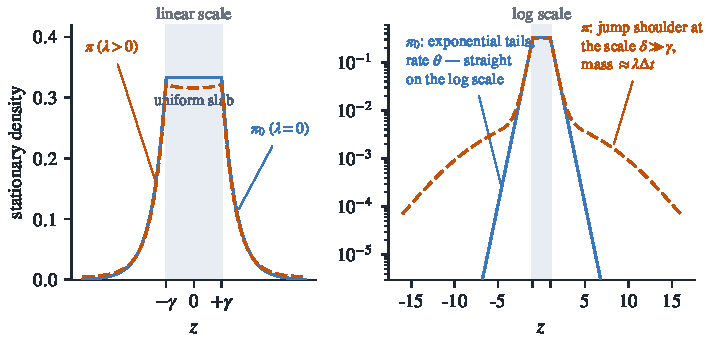
\includegraphics[width=\textwidth]{fig_stationary_law}
\caption{The stationary law of the pre-block mispricing on a linear (left) and
logarithmic (right) scale, at $\eta=2$, $\delta=5\gamma$, $\lambda\dt=0.08$.
The law $\pi_0$ ($\lambda=0$, the closed form \eqref{eq:pi0}) is uniform on the
band with exponential tails of rate $\theta$. With Merton jumps, $\pi$
(quasi-exact: jump feedback on the carried state is ignored, an $O(\lambda\dt)$
effect) adds a far field at the jump scale $\delta\gg\gamma$ --- the shoulder
leaving the exponential tail on the log scale, mass that no block schedule can
pull in. The slab of $\pi$ is also slightly depressed towards its centre:
exact uniformity on the band is a $\lambda=0$ property, and jumps break it at
$O(\lambda\dt)$, exaggerated here by the stylised $\lambda\dt$.}
\label{fig:statlaw}
\end{figure}
